\documentclass[twocolumn]{article}
\usepackage{graphicx}
\usepackage{amsmath}
\usepackage{hyperref}

\begin{document}
\title{Final Exam: Inverse iteration algorithm for eigenvalues}
\author{Simon Vendelbo Bylling Jensen\thanks{AU E-mail: 201507956@uni.au.dk} \thanks{CERN E-mail: simon.vendelbo.jensen@cern.ch}\\
Stud. Nr. 201507956 \\
Au Id. Au545766}
\date{\today}
\maketitle

\begin{abstract}
The  solution of exercise 10 for the final exam. An implementation f an inverse iteration algorithm for eigenvalues and eigenvectors. Such an implementation has been made, the first relying on a Golub-Kahan-Lanczos bidiagonalization iterating using a calculated inverse of the matrix, as well as a method using QR-decomposition by modified Gram-Schmidt orthogonalization to iterate through the solution of a linear system using backsubstitution. 
\end{abstract}

\section*{Introduction and Problem}
I have recieved exercise number 10, since my student number 56 by modulus 23 will give 10. The problem is to implement a variant of the inverse iteration method that calculates the eigenvalue closest to a given number $s$ and the corresponding eigenvector. The problem of finding eigenvalues and corresponding eigenvectors are crucial to various fields of physics and engineering. Especially for higly complicated quantum systems, complicated enginerring systems and much more, the task of finding an individual eigenvalue and determine its corresponding eigenvectors is essential. The algorithm, which will be demonstrated is a fast and effective way of doing excactly that. 

At first the implementation and theory of inverse iteration method the will be described in section \ref{sec:0} and afterwards the different related methods will be compared and analysed in section \ref{sec:5}. Implementations and simple calculations using the examined methods will similarly be demonstrated in the main.c file, and which results can be found in the out.txt file, as well as described hereafter. 

\section{\label{sec:0}Implementation and Theory}
The implementation and theory all relies on the lecture notes from ref. \cite[Chapter 12 - Eigenvalues 2: Power methods and Krylov subspace methods]{Dmi}. The refined inverse iteration method relies on a few simple principles. All of these principles will be described by different examples, which are all demonstrated in the main.c file, and which results can be found in the out.txt file. The description of the inverse iteration method will thereby be clear, by going through simpler implementations of the same procedure. This will be the case for sections \ref{sec:1, sec:2}. Hereafter first the implementation using a Golub-Kahan-Lanczos bidiagonalization will be described in section \ref{sec:3} at at last, the refined incerse iteration method will be described in section \ref{sec:4}.  

\subsection{\label{sec:1}The Power Method}
Since the inverse iteration method is a cleverly designed power method, it is essential to introduce the basics of the power methods. The simplest power method is the power iteration which works by multiplying a random vector $\vec{V}$ on a matrix $A$ of similar size, which we want to know the largest eigenvalue and corresponding eigenvector. By continiously multiplying the vector $\vec{V}$ on the matrix $A$, through the iteration
\begin{equation}
\vec{V}_{i+1} = A \vec{V}_i \label{eq:1}
\end{equation}
we are able to aproximate the largest eigenvector and largest eigenvalue very cleverly. The vector will at some point simply converge to the largest eigenvector. This is since by the multiplication, the dimension in which the eigenvector corresponding to the numerically largest eigenvalue will give the largest enhancement of the vector, $\vec{V}$, and for each iteration, this will have positive feedback and will at some point have $\vec{V}$ converge to some vector, which normalized will approximate that eigenvector. If the vector $\vec{V}$ will converge to the eigenvector, then at some point every iteration and thereby multiplicaltion will fullfill the eigenvector identity
\begin{equation}
A \vec{V}_\lambda = \lambda \vec{V}_\lambda \label{eq:2}
\end{equation}
We will thereby be able to approximate the largest eigenvalue continuously by finding the factor, in which V increases for every iteration. This parameter which are contiously detected are called the Rayleigh quotient, and will at one point converge to the largest eigenvalue. This is given as
\begin{equation}
\lambda \left[ \vec{V}_i \right] = \frac{\vec{V}^T_i A \vec{V}}{\vec{V}_i \cdot \vec{V}_i} \label{eq:3}
\end{equation}
For the implementation in main.c. the satisfaction critera for when an eigenvalue has been found, is when this Rayleigh quotient have converged and do not improve anymore with an iteration. This method is particularly effective in use, since it do not have to do any large matrix decompositions, which the computation of eigenvalues usually requires. 

\subsection{\label{sec:2}The Inverse Power method}
Intuitively, when one would be able to converge to the numerical largest eigenvalue by continuisly multiplying with the matrix $A$ one would expect, that a similar procedure could be done to find the numerically smallest eigenvalue. This is true, but the cost of this implementation, is the fact that one would in this case have to calculate the inverse of the matrix $A$. By the similar argument as for the power method, by multiplying with the inverse of $A$, the minimum eigenvalue, will now be dominant and the vector $\vec{V}$ will converge to the corresponding eigenvector. The iterations are hereby similar to equation \eqref{eq:1} and given as
\begin{equation}
\vec{V}_{i+1} = A^{-1} \vec{V}_i \label{eq:4}
\end{equation}

The inverse are for this case, found using the Golub-Kahan-Lanczos bidiagonalization as prevously implemented in the Linear Equation exercise C. This procedure is described in the following subsection \ref{sec:2.2}. When this is found, one can continiously apply itteration \ref{eq:4} to find the most dominant eigenvector when inverse iterating, corresponding to the eigenvector with the numerically smallet eigenvalue. This time since we apply the $A^{-1}$ instead of $A$, the eigenvector identity now becomes
\begin{equation}
 A^{-1} \vec{V}_\lambda = \frac{1}{\lambda} \vec{V}_\lambda \label{eq:5}
\end{equation}
instead of equation \eqref{eq:2}. And therefore the Rayleigh parameter from \eqref{eq:3} will not be approximating the lowest numerical eigenvalue, but instread its inverse. 
\subsubsection{\label{sec:2.2} Golub Kahan Lanczos bidiagonalization}
The Goloub-Kahan-Lanczos bidiagonalization is the subject of the previous exam exercise 9, and the linear-equation exercise C, this therby been made to use in this implementation as well. The procedure of implementing this is described in ref. \cite{BKL}. The method is usualy the start of a single value decomposition, and work by computing the unitary othogonal matricies $U$ and $V$, such that 
\begin{equation}
U^\ast A V = B,
\end{equation}
where $B$ is bidiagonal. This procedure is related the Gram-Schmidt procedure, since it starts with one vector in both $V$ and $U$ where it orthogonalize it to the previous vectors, it normalizes the vector, but furthermore than the simple Gram-Schmidt procedure, the Golub-Kahan-Lanczos bidiagonalization makes sure, through relations

\begin{align}
\alpha_k \vec{U}_{k} &= A\vec{V}_k - \beta_{k-1} \vec{U}_{k-1}, \\
\beta_k \vec{V}_{k+1} &= A^{\ast}\vec{U}_k - \alpha_k \vec{V}_k,
\end{align}
with $\alpha_k = \vec{U}_k^\ast A \vec{V}_k$ and $\beta_k = \vec{U}_k^\ast A \vec{V}_{k+1}$ that, where the Gram-Schmidt procedure will return a triangular matrix, which can be solved for finding the inverse through backpropagation, the Golub-Kahan-Lanczos returns a matrix $B$ for finding the inverse, that will be quicker to solve through backpropagation, since it is bidiagonal. The solution for the inverse, can thereby easily be found, by backsubstitution of the linear system
\begin{align}
A \cdot A^{-1} &= I,\\
U B V^T A^{-1} &= I,\\
B \left(V^T  A^{-1}\right) &= U^T.
\end{align}
This linear system is then solved for $V^T  A^{-1}$ which can then be multiplied with the orthogonal $V$ for finding the inverse. Many other aspects of this algorithm could be widely covered, but since this is not the point of the exercise, we will settle with the fact that the Golub-Kahan-Lanczos bidiagonalization procedure are able to provide us with $A^{-1}$ for the inverse power method.

\subsection{\label{sec:3} Shifted Inverse Iteration} 
Since we in the final iteration method, will want to estimate a eigenvalue with corresponding eigenvector, which relies closely to a given value $s$ which is not nessesarely the largest or the smallest eigenvalue. Then we need to implement a new method, that will converge to a wanted region of eigenvalues. This is done using the previous inverse iteration method, since it converges to a controlled value $0$, which will then has to be shifted to the given point $s$
 This can be simply done with an understanding of the linear algebra of eigenvalues and eigenvectors. If one apply the shift
\begin{equation}
A \rightarrow A - sI
\end{equation} 
Any eigenvectors of $A$ will on this shifted matrix still remain an eigenvector, but through equation \eqref{eq:2} give
\begin{align}
\left(A - s I\right) \vec{V}_\lambda &=  A \vec{V}_\lambda - s I \vec{V}_\lambda, \\
 &= \lambda \vec{V}_\lambda  -  s \vec{V}_\lambda, \\ 
 &= \left(\lambda - s\right) \vec{V}_\lambda. 
\end{align}
Thereby introducing a shifted eigenvalue of $\lambda \rightarrow \lambda - s$. By introducing this shift, one can simply use the inverse power procedure with iterations as
\begin{equation}
\vec{V}_{i+1} = \left(A - sI\right)^{-1} \vec{V}_i \label{eq:6}
\end{equation}

find any eigenvalues, with the expected eigenvalue area around $s$, in which this eigenvalue now will be shifted to be close to $0$ for the inverse power method to converge to it. Afterwards one must remember to shift eigenvalue back by the same $s$, to find its actual location, whereas the eigenvector remains the same. This procedure has been implemented and tested in the main.c file using Golub-Kahan-Lanczos bidiagonalization method to find the inverse of the shifted $\left( A - sI \right)^{-1}$.
A more refined way of doung the shifted inverse power method is the inverse iteration method, in which one do not need to calculate the inverse of $A$, but instead solves a linear system. This will now follow. 

\subsection{Inverse Iteration Method}
The main difference in the inverse power method and this refined inverse iteration method is the change from iteration through multiplication as in equation \eqref{eq:6}, to now iterate through finding the next vector by solving the linear system
\begin{equation}
\left(A - sI\right) \vec{V}_{i+1} =  \vec{V}_i \label{eq:6}
\end{equation}
This could in fact be done by the previously defined Golub-Kahan-Lanczos bidiagonalization method, since this will end up in a backsubstitution, which is significantly simple for the bidiagonalized matrices. However to demonstrate another procedure of solving theese systems, this time a simple QR-decomposition by modified Gram-Schmidt orthogonalization has been made as in the linear equation exercise B. This method will be discussed in the following subsection, but differs from the Golub-Kahan-Lanczos bidiagonalization method by being faster to compute initially, since it only needs to construct a single orthogonal matric. But since the trangular matrix from the QR decomposition is slower to make a complete backsubstitution of, than the quick backsubstitution of the bidiagonalized matrix, then the main differnce between theese two methods for this implementation. Is the QR-decomposition being quicker to initialize, but more costly per iteration, whereas the Golub-Kahan-Lanczos method is more costly to initialize, but quicker to run. Since we want to implement an algorithm, that allows the user to specify how often the system should replace the user provided $s$ with the estimated eigenvalue from the Rayleigh quotient, whereas the QR or Golub-Kahan-Lanczos method would be reinitialized, then for a demonstration of an inverse iteration algorithm with many continious updates, the QR-decomposition will be the fastest, and for one in which the user-supplied estimate is very well, and one would not need to replace it, with the estimate from the Rayleigh quotient, one would prefer the Golub-Kahan-Lanczos method. \\

In reference \cite{Dmi} it states that in practise the method is usually used for finding a result when a good approximation for the eigenvalue is known, with only a few iterations. If only a few iterations shall be made, then the fast initializing QR-decomposition will be the fastest, and therefore the one i will choose for the iteration procedure. 

The QR-decomposition will be described in the following section \ref{sec3.2}, and will through backsubstitution determine the new vector at each iteration. With the optimized iteration step, the rest of the inverse iteration method is simple implemented as for the shifted inverse power method as described in section \ref{sec:2}.

\subsubsection{\label{sec:3.2}QR-Decomposition by modified Gram-Schmidt orthogonalization}
 
 




  \begin{figure}[h]
% GNUPLOT: LaTeX picture with Postscript
\begingroup
  \makeatletter
  \providecommand\color[2][]{%
    \GenericError{(gnuplot) \space\space\space\@spaces}{%
      Package color not loaded in conjunction with
      terminal option `colourtext'%
    }{See the gnuplot documentation for explanation.%
    }{Either use 'blacktext' in gnuplot or load the package
      color.sty in LaTeX.}%
    \renewcommand\color[2][]{}%
  }%
  \providecommand\includegraphics[2][]{%
    \GenericError{(gnuplot) \space\space\space\@spaces}{%
      Package graphicx or graphics not loaded%
    }{See the gnuplot documentation for explanation.%
    }{The gnuplot epslatex terminal needs graphicx.sty or graphics.sty.}%
    \renewcommand\includegraphics[2][]{}%
  }%
  \providecommand\rotatebox[2]{#2}%
  \@ifundefined{ifGPcolor}{%
    \newif\ifGPcolor
    \GPcolortrue
  }{}%
  \@ifundefined{ifGPblacktext}{%
    \newif\ifGPblacktext
    \GPblacktexttrue
  }{}%
  % define a \g@addto@macro without @ in the name:
  \let\gplgaddtomacro\g@addto@macro
  % define empty templates for all commands taking text:
  \gdef\gplbacktext{}%
  \gdef\gplfronttext{}%
  \makeatother
  \ifGPblacktext
    % no textcolor at all
    \def\colorrgb#1{}%
    \def\colorgray#1{}%
  \else
    % gray or color?
    \ifGPcolor
      \def\colorrgb#1{\color[rgb]{#1}}%
      \def\colorgray#1{\color[gray]{#1}}%
      \expandafter\def\csname LTw\endcsname{\color{white}}%
      \expandafter\def\csname LTb\endcsname{\color{black}}%
      \expandafter\def\csname LTa\endcsname{\color{black}}%
      \expandafter\def\csname LT0\endcsname{\color[rgb]{1,0,0}}%
      \expandafter\def\csname LT1\endcsname{\color[rgb]{0,1,0}}%
      \expandafter\def\csname LT2\endcsname{\color[rgb]{0,0,1}}%
      \expandafter\def\csname LT3\endcsname{\color[rgb]{1,0,1}}%
      \expandafter\def\csname LT4\endcsname{\color[rgb]{0,1,1}}%
      \expandafter\def\csname LT5\endcsname{\color[rgb]{1,1,0}}%
      \expandafter\def\csname LT6\endcsname{\color[rgb]{0,0,0}}%
      \expandafter\def\csname LT7\endcsname{\color[rgb]{1,0.3,0}}%
      \expandafter\def\csname LT8\endcsname{\color[rgb]{0.5,0.5,0.5}}%
    \else
      % gray
      \def\colorrgb#1{\color{black}}%
      \def\colorgray#1{\color[gray]{#1}}%
      \expandafter\def\csname LTw\endcsname{\color{white}}%
      \expandafter\def\csname LTb\endcsname{\color{black}}%
      \expandafter\def\csname LTa\endcsname{\color{black}}%
      \expandafter\def\csname LT0\endcsname{\color{black}}%
      \expandafter\def\csname LT1\endcsname{\color{black}}%
      \expandafter\def\csname LT2\endcsname{\color{black}}%
      \expandafter\def\csname LT3\endcsname{\color{black}}%
      \expandafter\def\csname LT4\endcsname{\color{black}}%
      \expandafter\def\csname LT5\endcsname{\color{black}}%
      \expandafter\def\csname LT6\endcsname{\color{black}}%
      \expandafter\def\csname LT7\endcsname{\color{black}}%
      \expandafter\def\csname LT8\endcsname{\color{black}}%
    \fi
  \fi
    \setlength{\unitlength}{0.0500bp}%
    \ifx\gptboxheight\undefined%
      \newlength{\gptboxheight}%
      \newlength{\gptboxwidth}%
      \newsavebox{\gptboxtext}%
    \fi%
    \setlength{\fboxrule}{0.5pt}%
    \setlength{\fboxsep}{1pt}%
\begin{picture}(4320.00,3456.00)%
    \gplgaddtomacro\gplbacktext{%
      \csname LTb\endcsname%%
      \put(645,669){\makebox(0,0)[r]{\strut{}$0$}}%
      \csname LTb\endcsname%%
      \put(645,994){\makebox(0,0)[r]{\strut{}$100$}}%
      \csname LTb\endcsname%%
      \put(645,1319){\makebox(0,0)[r]{\strut{}$200$}}%
      \csname LTb\endcsname%%
      \put(645,1644){\makebox(0,0)[r]{\strut{}$300$}}%
      \csname LTb\endcsname%%
      \put(645,1969){\makebox(0,0)[r]{\strut{}$400$}}%
      \csname LTb\endcsname%%
      \put(645,2294){\makebox(0,0)[r]{\strut{}$500$}}%
      \csname LTb\endcsname%%
      \put(645,2619){\makebox(0,0)[r]{\strut{}$600$}}%
      \csname LTb\endcsname%%
      \put(645,2944){\makebox(0,0)[r]{\strut{}$700$}}%
      \csname LTb\endcsname%%
      \put(645,3269){\makebox(0,0)[r]{\strut{}$800$}}%
      \csname LTb\endcsname%%
      \put(821,409){\makebox(0,0){\strut{}$0$}}%
      \csname LTb\endcsname%%
      \put(1341,409){\makebox(0,0){\strut{}$5$}}%
      \csname LTb\endcsname%%
      \put(1860,409){\makebox(0,0){\strut{}$10$}}%
      \csname LTb\endcsname%%
      \put(2380,409){\makebox(0,0){\strut{}$15$}}%
      \csname LTb\endcsname%%
      \put(2900,409){\makebox(0,0){\strut{}$20$}}%
      \csname LTb\endcsname%%
      \put(3419,409){\makebox(0,0){\strut{}$25$}}%
      \csname LTb\endcsname%%
      \put(3939,409){\makebox(0,0){\strut{}$30$}}%
    }%
    \gplgaddtomacro\gplfronttext{%
      \csname LTb\endcsname%%
      \put(153,1969){\rotatebox{-270}{\makebox(0,0){\strut{}Number of Iterations}}}%
      \csname LTb\endcsname%%
      \put(2380,130){\makebox(0,0){\strut{}Matrix Dimension "n"}}%
      \csname LTb\endcsname%%
      \put(3065,3102){\makebox(0,0)[r]{\strut{}Power Iter.}}%
      \csname LTb\endcsname%%
      \put(3065,2916){\makebox(0,0)[r]{\strut{}Inverse Power Iter.}}%
      \csname LTb\endcsname%%
      \put(3065,2730){\makebox(0,0)[r]{\strut{}Shifted Inverse Iter.}}%
      \csname LTb\endcsname%%
      \put(3065,2544){\makebox(0,0)[r]{\strut{}Inverse Iter.}}%
    }%
    \gplbacktext
    \put(0,0){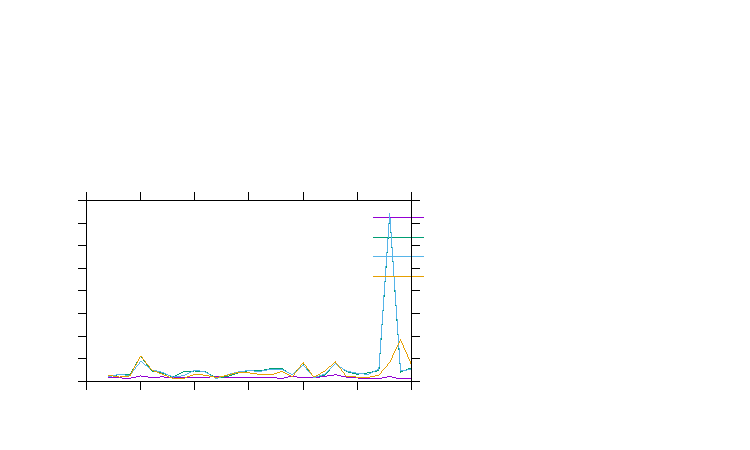
\includegraphics{plot-cairo}}%
    \gplfronttext
  \end{picture}%
\endgroup

\caption{Comparison between the calculated arctangent function using the differential equation found in "myarctan.c" and the arctangent function from the math.h library.}
\label{fig-atan}
\end{figure}

  \begin{figure}[h]
% GNUPLOT: LaTeX picture with Postscript
\begingroup
  \makeatletter
  \providecommand\color[2][]{%
    \GenericError{(gnuplot) \space\space\space\@spaces}{%
      Package color not loaded in conjunction with
      terminal option `colourtext'%
    }{See the gnuplot documentation for explanation.%
    }{Either use 'blacktext' in gnuplot or load the package
      color.sty in LaTeX.}%
    \renewcommand\color[2][]{}%
  }%
  \providecommand\includegraphics[2][]{%
    \GenericError{(gnuplot) \space\space\space\@spaces}{%
      Package graphicx or graphics not loaded%
    }{See the gnuplot documentation for explanation.%
    }{The gnuplot epslatex terminal needs graphicx.sty or graphics.sty.}%
    \renewcommand\includegraphics[2][]{}%
  }%
  \providecommand\rotatebox[2]{#2}%
  \@ifundefined{ifGPcolor}{%
    \newif\ifGPcolor
    \GPcolortrue
  }{}%
  \@ifundefined{ifGPblacktext}{%
    \newif\ifGPblacktext
    \GPblacktexttrue
  }{}%
  % define a \g@addto@macro without @ in the name:
  \let\gplgaddtomacro\g@addto@macro
  % define empty templates for all commands taking text:
  \gdef\gplbacktext{}%
  \gdef\gplfronttext{}%
  \makeatother
  \ifGPblacktext
    % no textcolor at all
    \def\colorrgb#1{}%
    \def\colorgray#1{}%
  \else
    % gray or color?
    \ifGPcolor
      \def\colorrgb#1{\color[rgb]{#1}}%
      \def\colorgray#1{\color[gray]{#1}}%
      \expandafter\def\csname LTw\endcsname{\color{white}}%
      \expandafter\def\csname LTb\endcsname{\color{black}}%
      \expandafter\def\csname LTa\endcsname{\color{black}}%
      \expandafter\def\csname LT0\endcsname{\color[rgb]{1,0,0}}%
      \expandafter\def\csname LT1\endcsname{\color[rgb]{0,1,0}}%
      \expandafter\def\csname LT2\endcsname{\color[rgb]{0,0,1}}%
      \expandafter\def\csname LT3\endcsname{\color[rgb]{1,0,1}}%
      \expandafter\def\csname LT4\endcsname{\color[rgb]{0,1,1}}%
      \expandafter\def\csname LT5\endcsname{\color[rgb]{1,1,0}}%
      \expandafter\def\csname LT6\endcsname{\color[rgb]{0,0,0}}%
      \expandafter\def\csname LT7\endcsname{\color[rgb]{1,0.3,0}}%
      \expandafter\def\csname LT8\endcsname{\color[rgb]{0.5,0.5,0.5}}%
    \else
      % gray
      \def\colorrgb#1{\color{black}}%
      \def\colorgray#1{\color[gray]{#1}}%
      \expandafter\def\csname LTw\endcsname{\color{white}}%
      \expandafter\def\csname LTb\endcsname{\color{black}}%
      \expandafter\def\csname LTa\endcsname{\color{black}}%
      \expandafter\def\csname LT0\endcsname{\color{black}}%
      \expandafter\def\csname LT1\endcsname{\color{black}}%
      \expandafter\def\csname LT2\endcsname{\color{black}}%
      \expandafter\def\csname LT3\endcsname{\color{black}}%
      \expandafter\def\csname LT4\endcsname{\color{black}}%
      \expandafter\def\csname LT5\endcsname{\color{black}}%
      \expandafter\def\csname LT6\endcsname{\color{black}}%
      \expandafter\def\csname LT7\endcsname{\color{black}}%
      \expandafter\def\csname LT8\endcsname{\color{black}}%
    \fi
  \fi
    \setlength{\unitlength}{0.0500bp}%
    \ifx\gptboxheight\undefined%
      \newlength{\gptboxheight}%
      \newlength{\gptboxwidth}%
      \newsavebox{\gptboxtext}%
    \fi%
    \setlength{\fboxrule}{0.5pt}%
    \setlength{\fboxsep}{1pt}%
\begin{picture}(4320.00,3456.00)%
    \gplgaddtomacro\gplbacktext{%
      \csname LTb\endcsname%%
      \put(543,669){\makebox(0,0)[r]{\strut{}$10$}}%
      \csname LTb\endcsname%%
      \put(543,975){\makebox(0,0)[r]{\strut{}$20$}}%
      \csname LTb\endcsname%%
      \put(543,1281){\makebox(0,0)[r]{\strut{}$30$}}%
      \csname LTb\endcsname%%
      \put(543,1587){\makebox(0,0)[r]{\strut{}$40$}}%
      \csname LTb\endcsname%%
      \put(543,1893){\makebox(0,0)[r]{\strut{}$50$}}%
      \csname LTb\endcsname%%
      \put(543,2198){\makebox(0,0)[r]{\strut{}$60$}}%
      \csname LTb\endcsname%%
      \put(543,2504){\makebox(0,0)[r]{\strut{}$70$}}%
      \csname LTb\endcsname%%
      \put(543,2810){\makebox(0,0)[r]{\strut{}$80$}}%
      \csname LTb\endcsname%%
      \put(543,3116){\makebox(0,0)[r]{\strut{}$90$}}%
      \csname LTb\endcsname%%
      \put(719,409){\makebox(0,0){\strut{}$2$}}%
      \csname LTb\endcsname%%
      \put(1179,409){\makebox(0,0){\strut{}$3$}}%
      \csname LTb\endcsname%%
      \put(1639,409){\makebox(0,0){\strut{}$4$}}%
      \csname LTb\endcsname%%
      \put(2099,409){\makebox(0,0){\strut{}$5$}}%
      \csname LTb\endcsname%%
      \put(2559,409){\makebox(0,0){\strut{}$6$}}%
      \csname LTb\endcsname%%
      \put(3019,409){\makebox(0,0){\strut{}$7$}}%
      \csname LTb\endcsname%%
      \put(3479,409){\makebox(0,0){\strut{}$8$}}%
      \csname LTb\endcsname%%
      \put(3939,409){\makebox(0,0){\strut{}$9$}}%
    }%
    \gplgaddtomacro\gplfronttext{%
      \csname LTb\endcsname%%
      \put(153,1969){\rotatebox{-270}{\makebox(0,0){\strut{}Number of iterations}}}%
      \csname LTb\endcsname%%
      \put(2329,130){\makebox(0,0){\strut{}Matrix Dimension "n"}}%
      \csname LTb\endcsname%%
      \put(2657,3102){\makebox(0,0)[r]{\strut{}20 Iter. per. Upd.}}%
      \csname LTb\endcsname%%
      \put(2657,2916){\makebox(0,0)[r]{\strut{}40 Iter. per. Upd.}}%
      \csname LTb\endcsname%%
      \put(2657,2730){\makebox(0,0)[r]{\strut{}60 Iter. per. Upd.}}%
      \csname LTb\endcsname%%
      \put(2657,2544){\makebox(0,0)[r]{\strut{}80 Iter. per. Upd.}}%
    }%
    \gplbacktext
    \put(0,0){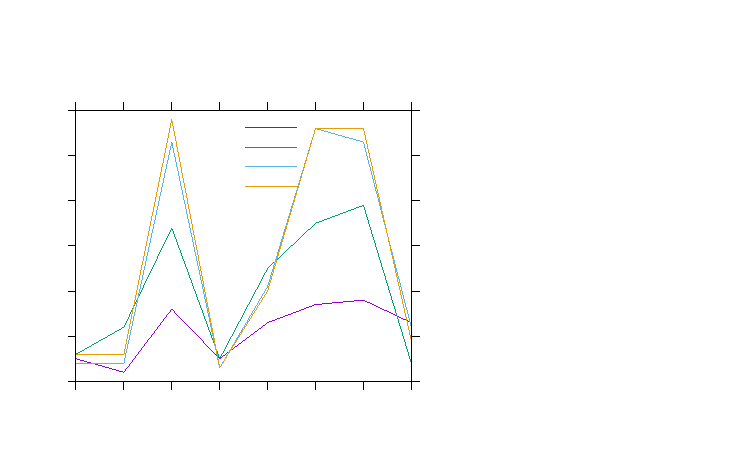
\includegraphics{plot-cairo-2}}%
    \gplfronttext
  \end{picture}%
\endgroup

\caption{Comparison between the calculated arctangent function using the differential equation found in "myarctan.c" and the arctangent function from the math.h library.}
\label{fig-atan}
\end{figure}


\begin{figure}[h]
% GNUPLOT: LaTeX picture with Postscript
\begingroup
  \makeatletter
  \providecommand\color[2][]{%
    \GenericError{(gnuplot) \space\space\space\@spaces}{%
      Package color not loaded in conjunction with
      terminal option `colourtext'%
    }{See the gnuplot documentation for explanation.%
    }{Either use 'blacktext' in gnuplot or load the package
      color.sty in LaTeX.}%
    \renewcommand\color[2][]{}%
  }%
  \providecommand\includegraphics[2][]{%
    \GenericError{(gnuplot) \space\space\space\@spaces}{%
      Package graphicx or graphics not loaded%
    }{See the gnuplot documentation for explanation.%
    }{The gnuplot epslatex terminal needs graphicx.sty or graphics.sty.}%
    \renewcommand\includegraphics[2][]{}%
  }%
  \providecommand\rotatebox[2]{#2}%
  \@ifundefined{ifGPcolor}{%
    \newif\ifGPcolor
    \GPcolortrue
  }{}%
  \@ifundefined{ifGPblacktext}{%
    \newif\ifGPblacktext
    \GPblacktexttrue
  }{}%
  % define a \g@addto@macro without @ in the name:
  \let\gplgaddtomacro\g@addto@macro
  % define empty templates for all commands taking text:
  \gdef\gplbacktext{}%
  \gdef\gplfronttext{}%
  \makeatother
  \ifGPblacktext
    % no textcolor at all
    \def\colorrgb#1{}%
    \def\colorgray#1{}%
  \else
    % gray or color?
    \ifGPcolor
      \def\colorrgb#1{\color[rgb]{#1}}%
      \def\colorgray#1{\color[gray]{#1}}%
      \expandafter\def\csname LTw\endcsname{\color{white}}%
      \expandafter\def\csname LTb\endcsname{\color{black}}%
      \expandafter\def\csname LTa\endcsname{\color{black}}%
      \expandafter\def\csname LT0\endcsname{\color[rgb]{1,0,0}}%
      \expandafter\def\csname LT1\endcsname{\color[rgb]{0,1,0}}%
      \expandafter\def\csname LT2\endcsname{\color[rgb]{0,0,1}}%
      \expandafter\def\csname LT3\endcsname{\color[rgb]{1,0,1}}%
      \expandafter\def\csname LT4\endcsname{\color[rgb]{0,1,1}}%
      \expandafter\def\csname LT5\endcsname{\color[rgb]{1,1,0}}%
      \expandafter\def\csname LT6\endcsname{\color[rgb]{0,0,0}}%
      \expandafter\def\csname LT7\endcsname{\color[rgb]{1,0.3,0}}%
      \expandafter\def\csname LT8\endcsname{\color[rgb]{0.5,0.5,0.5}}%
    \else
      % gray
      \def\colorrgb#1{\color{black}}%
      \def\colorgray#1{\color[gray]{#1}}%
      \expandafter\def\csname LTw\endcsname{\color{white}}%
      \expandafter\def\csname LTb\endcsname{\color{black}}%
      \expandafter\def\csname LTa\endcsname{\color{black}}%
      \expandafter\def\csname LT0\endcsname{\color{black}}%
      \expandafter\def\csname LT1\endcsname{\color{black}}%
      \expandafter\def\csname LT2\endcsname{\color{black}}%
      \expandafter\def\csname LT3\endcsname{\color{black}}%
      \expandafter\def\csname LT4\endcsname{\color{black}}%
      \expandafter\def\csname LT5\endcsname{\color{black}}%
      \expandafter\def\csname LT6\endcsname{\color{black}}%
      \expandafter\def\csname LT7\endcsname{\color{black}}%
      \expandafter\def\csname LT8\endcsname{\color{black}}%
    \fi
  \fi
    \setlength{\unitlength}{0.0500bp}%
    \ifx\gptboxheight\undefined%
      \newlength{\gptboxheight}%
      \newlength{\gptboxwidth}%
      \newsavebox{\gptboxtext}%
    \fi%
    \setlength{\fboxrule}{0.5pt}%
    \setlength{\fboxsep}{1pt}%
\begin{picture}(4320.00,2592.00)%
    \gplgaddtomacro\gplbacktext{%
      \csname LTb\endcsname%%
      \put(645,669){\makebox(0,0)[r]{\strut{}$0$}}%
      \csname LTb\endcsname%%
      \put(645,862){\makebox(0,0)[r]{\strut{}$0.5$}}%
      \csname LTb\endcsname%%
      \put(645,1055){\makebox(0,0)[r]{\strut{}$1$}}%
      \csname LTb\endcsname%%
      \put(645,1248){\makebox(0,0)[r]{\strut{}$1.5$}}%
      \csname LTb\endcsname%%
      \put(645,1441){\makebox(0,0)[r]{\strut{}$2$}}%
      \csname LTb\endcsname%%
      \put(645,1633){\makebox(0,0)[r]{\strut{}$2.5$}}%
      \csname LTb\endcsname%%
      \put(645,1826){\makebox(0,0)[r]{\strut{}$3$}}%
      \csname LTb\endcsname%%
      \put(645,2019){\makebox(0,0)[r]{\strut{}$3.5$}}%
      \csname LTb\endcsname%%
      \put(645,2212){\makebox(0,0)[r]{\strut{}$4$}}%
      \csname LTb\endcsname%%
      \put(645,2405){\makebox(0,0)[r]{\strut{}$4.5$}}%
      \csname LTb\endcsname%%
      \put(821,409){\makebox(0,0){\strut{}$100$}}%
      \csname LTb\endcsname%%
      \put(1266,409){\makebox(0,0){\strut{}$200$}}%
      \csname LTb\endcsname%%
      \put(1712,409){\makebox(0,0){\strut{}$300$}}%
      \csname LTb\endcsname%%
      \put(2157,409){\makebox(0,0){\strut{}$400$}}%
      \csname LTb\endcsname%%
      \put(2603,409){\makebox(0,0){\strut{}$500$}}%
      \csname LTb\endcsname%%
      \put(3048,409){\makebox(0,0){\strut{}$600$}}%
      \csname LTb\endcsname%%
      \put(3494,409){\makebox(0,0){\strut{}$700$}}%
      \csname LTb\endcsname%%
      \put(3939,409){\makebox(0,0){\strut{}$800$}}%
    }%
    \gplgaddtomacro\gplfronttext{%
      \csname LTb\endcsname%%
      \put(153,1537){\rotatebox{-270}{\makebox(0,0){\strut{}y}}}%
      \csname LTb\endcsname%%
      \put(2380,130){\makebox(0,0){\strut{}x}}%
      \csname LTb\endcsname%%
      \put(2657,2238){\makebox(0,0)[r]{\strut{}Inverse Iteration}}%
      \csname LTb\endcsname%%
      \put(2657,2052){\makebox(0,0)[r]{\strut{}Jacobi Diag.}}%
    }%
    \gplbacktext
    \put(0,0){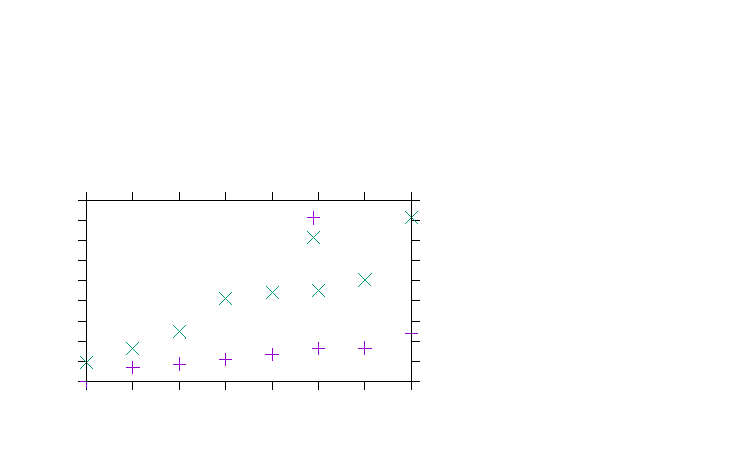
\includegraphics{plot-cairo_time}}%
    \gplfronttext
  \end{picture}%
\endgroup

\caption{Examination of the computing time as a function of....}
\label{fig-atan}
\end{figure}

\begin{thebibliography}{9}

\bibitem{GKL}
  Dongarra, J.
  \textit{Golub-Kahan-Lanczos Bidiagonalization Procedure.},
  \href{http://www.netlib.org/utk/people/JackDongarra/etemplates/node198.html}{Netbib.org/...},
  2019.
  
\bibitem{Dmi}
  Fedorov, D.V.
  \textit{Introduction to Numercal Methods},
  Lecture Notes, Aarhus University,
  2019.


\end{thebibliography}

\end{document}
